\documentclass{standalone}
\usepackage{tikz}

\begin{document}

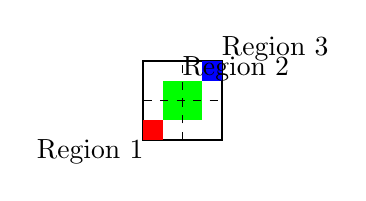
\begin{tikzpicture}[scale=0.5]
    % Draw the domain Omega
    \draw[thick] (-1,-1) rectangle (1,1);
    
    % Define colors for different regions
    \definecolor{region1}{RGB}{255,0,0} % Red
    \definecolor{region2}{RGB}{0,255,0} % Green
    \definecolor{region3}{RGB}{0,0,255} % Blue
    
    % Fill the regions with different colors
    \fill[region1] (-1,-1) rectangle (-0.5,-0.5);
    \fill[region2] (-0.5,-0.5) rectangle (0.5,0.5);
    \fill[region3] (0.5,0.5) rectangle (1,1);
    
    % Add labels for the regions
    \node at (-0.75,-0.75) [below left] {Region 1};
    \node at (-0.25,0.25) [above right] {Region 2};
    \node at (0.75,0.75) [above right] {Region 3};
    
    % Draw grid lines for better visualization
    \draw[dashed] (-1,0) -- (1,0);
    \draw[dashed] (0,-1) -- (0,1);
\end{tikzpicture}

\end{document}